\section{rSLA DSL}
\label{sec:dsl}
alphabet, vocabulary, language structure

production rules

\subsection{rSLA language structure, alphabet}

The rSLA language follows the semantic decomposition of the WSLA specification \cite{wsla}, where an SLA takes the form of a hierarchical tree with a single root node and numerous uni-directional edges. In an rSLA tree, the root node represents an SLA object. Figure \ref{rSLA_diag} illustrates diagrammatically the rSLA vocabulary as a tree of objects that the DSL implements. Listing \ref{lst} explains the rSLA tree using set notation to highlight the nesting between language objects. Such nesting is inherited from the WSLA specification \cite{wsla}.

\begin{minipage}{0.5\textwidth}
\begin{figure}[H]
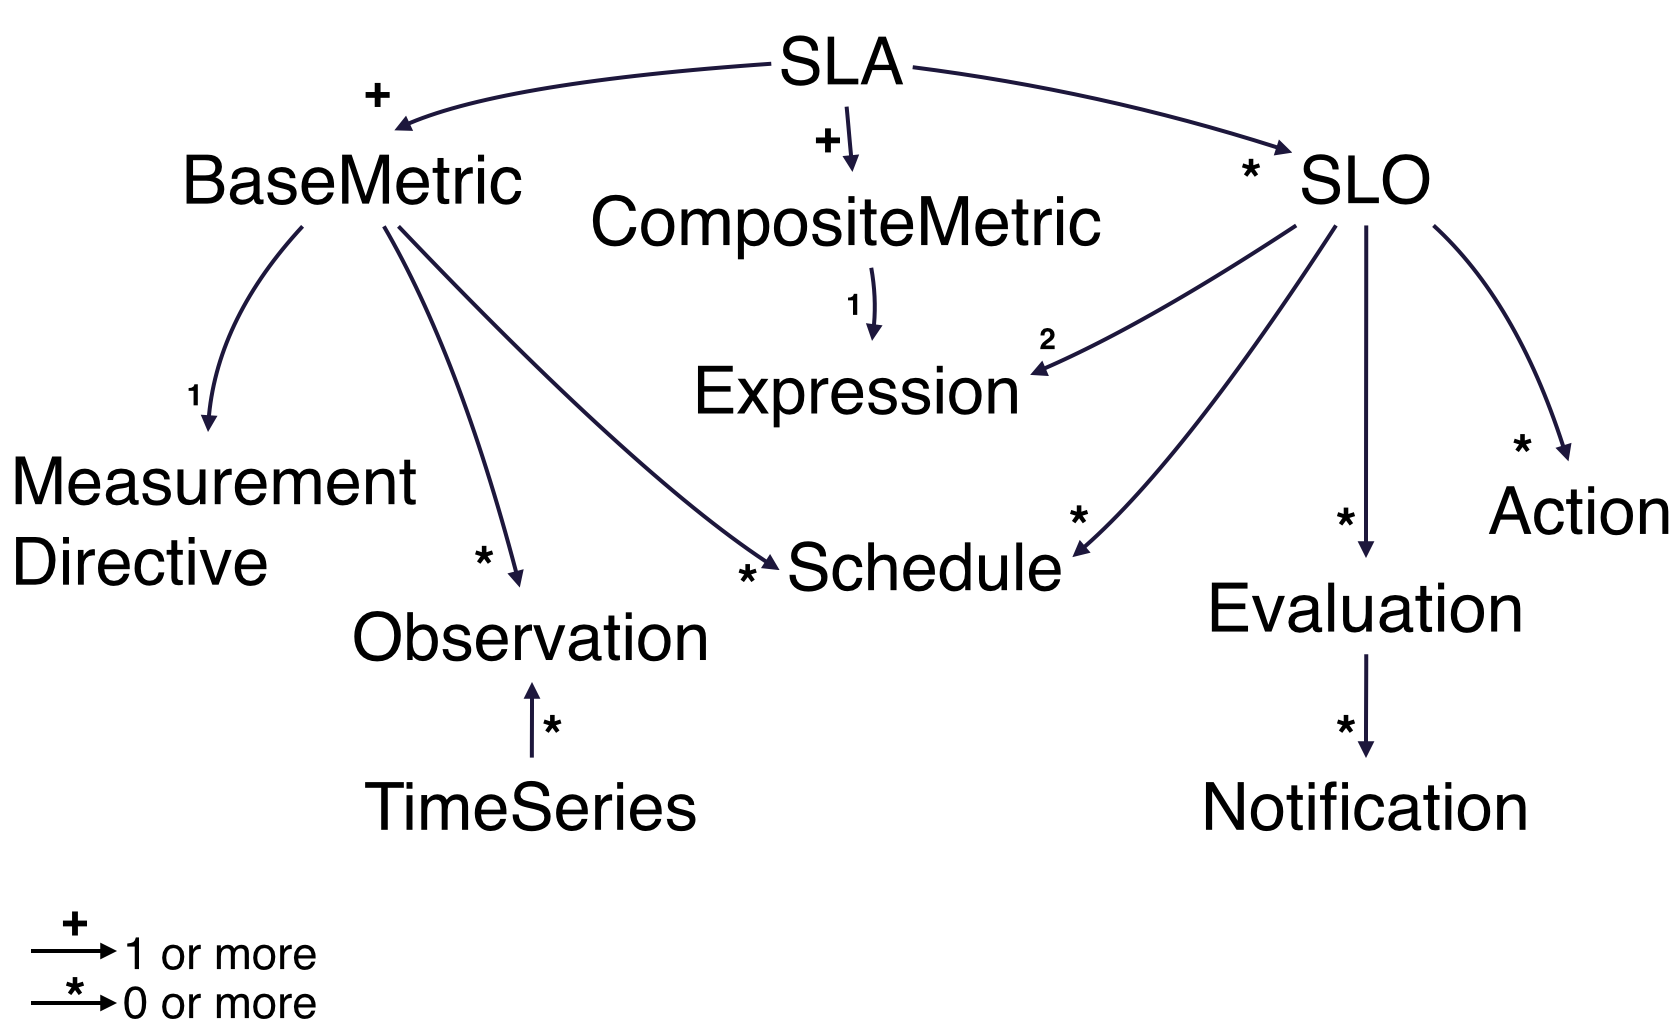
\includegraphics[width=1.0\textwidth]{pics/rslaobject}
\caption{\label{rslaobject} rSLA DSL object diagram}
\end{figure}
\end{minipage} \hfill
\begin{minipage}{0.5\textwidth}
\begin{lstlisting}[breaklines, mathescape, firstnumber=auto, caption=rSLA vocabulary, label=lst]
SLA $\supset$ { BaseMetric+, CompositeMetric*, SLO+ }
BaseMetric $\supset$ { MeasurementDirective, Observation*, Schedule* }
CompositeMetric $\supset$ { Expression* }
SLO $\supset$ { Expression*, Action*, Evaluation*, Schedule* }
\end{lstlisting}
\end{minipage}

Nodes that are close to the tree root in Figure \ref{rslaobject}, designate SLA branches like base, composite metrics and service level objectives. Edges between nodes are uni-directed to illustrate the rSLA tree hierarchy. The edge direction points to the nested element in the hierarchical relationship. 
Edges in Figure \ref{rslaobject} are labeled with +, * or number symbols to indicate that the multiplicity of nested objects. Hence, an SLA can be defined by sets of base, composite metric and SLO objects.

In the rSLA alphabet nested relationships denote inclusive associations between objects. For example, an SLA includes base, composite metrics as well as SLOs. As shown in Figure \ref{rslaobject}, edges between  rSLA objects do not share same multiplicity rules. The rSLA DSL follows the WSLA 
specification \cite{wsla} with respect to the definition of rSLA objects and of their basic attributes.

rSLA notification and timeSeries objects are not initially required to build and run SLA instances in a cloud environment, but may be required while one or more SLA management tasks are processed. Such objects are created by service level management operations like statistical analysis of data coming from monitoring or automated notification reports on scheduled events of service level evaluation. 

The rSLA DSL exposes such objects as structured programming blocks that a user can edit and modify according to specific needs. A user can also specify new elements for the rSLA vocabulary by integrating their definition in the rSLA programming library. The use and characteristics of rSLA programming blocks are analyzed in Section ??

\subsection{rSLA language production rules}

rSLA language constructs: elements have relationships/dependencies, there is nesting and management dependencies

production rules

\subsection{rSLA editing}